% Nicholas M. Rathmann <rathmann@nbi.ku.dk>

\documentclass[border=1pt,tikz]{standalone}

\usepackage{pgfplots,physics}
\usepackage{newtxtext,newtxmath} % RSPA-like font
\usetikzlibrary{calc,arrows.meta,decorations.markings}

\usepackage{xcolor}

\definecolor{dblue}{HTML}{08519c}
\definecolor{dred}{HTML}{a50f15}

\definecolor{cray1}{HTML}{b35806}
\definecolor{cray2}{HTML}{542788}

\definecolor{cfirn}{HTML}{f0f0f0}
\definecolor{cice}{HTML}{dcf0fd}
\definecolor{cbed}{HTML}{c9b1a2}

\tikzstyle{iceshading}=[top color=cice!200, bottom color=cice!90]
\tikzstyle{bedshading}=[top color=cbed, bottom color=cbed!160]
\tikzstyle{firnshading}=[top color=cfirn, bottom color=cfirn!250]

\tikzset{
	every picture/.style={font=\fontsize{9.1}{9.1}\selectfont,},
	anno/.style={font=\fontsize{8.5}{8.5}\selectfont,},
  	lw/.style={line width=0.9pt,},
	%%%
  	bed/.style={black, bedshading},
  	bedtop/.style={black!50, lw},
  	icesheet/.style={dblue, iceshading},
  	firn/.style={firnshading},
  	bubb/.style={gray,fill=white,line width=0.6pt},
	%%%
	CMPdot/.style={dred, fill=dred, lw}, 
	ray1/.style={lw, cray1, densely dashed},
	ray2/.style={lw, cray2},
	reflector/.style={dblue}, 
	axis/.style={black, lw, -{Latex[scale=0.9]}, line cap=rect,},
	decoration={markings, 
		mark=at position 0.3 with {\arrow{Latex[scale=1.1]}},
		mark=at position 0.7 with {\arrow{Latex[scale=1.1]}}
	},
}

\gdef\W{7cm}      % width
\gdef\H{1.8cm}    % ice thickness
\gdef\Hf{1cm}     % firn thickness
\gdef\Hbed{0.5cm} % bed thickness
\gdef\Hrfl{0.3cm} % reflector level

\gdef\xT{\W/2 * 0.65}

\begin{document}
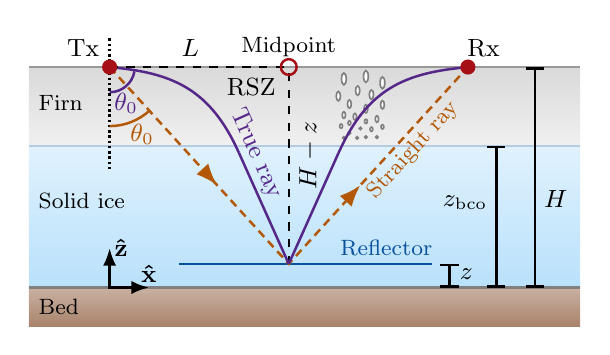
\begin{tikzpicture}[]

	%%% Firn, ice, bed

	\begin{scope}[xshift=0.2cm]

		\fill[firn, shading angle=180] ({-\W/2},\H) rectangle ++(\W,\Hf);	
		\draw[lw, gray!80] (-\W/2,{\H+\Hf}) -- ++(\W,0);
		\node[anchor=west,anno] at (-1*\W/2,\H+\Hf-1.3em) {Firn};
				
		\fill[icesheet, shading angle=180] ({-\W/2},0) rectangle ++(\W,\H);
		\draw[lw, dblue!30] (-\W/2,\H) -- ++(\W,0);
		\node[anchor=west,anno] at (-1*\W/2,\H-2.0em) {Solid ice};
		
		\fill[bed] (-\W/2,-1*\Hbed) rectangle ++ (\W,\Hbed);
		\draw[bedtop] (-\W/2,0) -- ++(\W,0);
		\node[anchor=west,anno] at (-1*\W/2,-0.7em) {Bed};

	\end{scope}
	
	%%% Bubbles
	
	\gdef\bw{0.03cm}
	
	\gdef\bs{1}
	\gdef\be{2.5}
	\draw[bubb] (\W*0.14, {\H+0.88*\Hf}) ellipse ({\bs*\bw} and {\bs*\bw*\be});	
	\draw[bubb] (\W*0.10, {\H+0.85*\Hf}) ellipse ({\bs*\bw} and {\bs*\bw*\be});	
	\draw[bubb] (\W*0.17, {\H+0.80*\Hf}) ellipse ({\bs*\bw} and {\bs*\bw*\be});	
	\gdef\bs{0.9}
	\gdef\be{2.2}
	\draw[bubb] (\W*0.125, {\H+0.70*\Hf}) ellipse  ({\bs*\bw} and {\bs*\bw*\be});	
	\draw[bubb] (\W*0.15, {\H+0.65*\Hf}) ellipse  ({\bs*\bw} and {\bs*\bw*\be});	
	\draw[bubb] (\W*0.09, {\H+0.63*\Hf}) ellipse  ({\bs*\bw} and {\bs*\bw*\be});	
	\gdef\bs{0.8}
	\draw[bubb] (\W*0.11, {\H+0.53*\Hf}) ellipse  ({\bs*\bw} and {\bs*\bw*\be});	
	\draw[bubb] (\W*0.14, {\H+0.47*\Hf}) ellipse  ({\bs*\bw} and {\bs*\bw*\be});	
	\draw[bubb] (\W*0.17, {\H+0.52*\Hf}) ellipse  ({\bs*\bw} and {\bs*\bw*\be});	
	\gdef\bs{0.7}
	\gdef\be{2}
	\draw[bubb] (\W*0.10, {\H+0.39*\Hf}) ellipse  ({\bs*\bw} and {\bs*\bw*\be});	
	\draw[bubb] (\W*0.12, {\H+0.37*\Hf}) ellipse  ({\bs*\bw} and {\bs*\bw*\be});	
	\draw[bubb] (\W*0.16, {\H+0.34*\Hf}) ellipse  ({\bs*\bw} and {\bs*\bw*\be});	
	\gdef\bs{0.6}
	\gdef\be{1.5}
	\draw[bubb] (\W*0.095, {\H+0.25*\Hf}) ellipse  ({\bs*\bw} and {\bs*\bw*\be});	
	\draw[bubb] (\W*0.11, {\H+0.29*\Hf}) ellipse  ({\bs*\bw} and {\bs*\bw*\be});	
	\draw[bubb] (\W*0.14, {\H+0.31*\Hf}) ellipse  ({\bs*\bw} and {\bs*\bw*\be});	
	\draw[bubb] (\W*0.15, {\H+0.21*\Hf}) ellipse  ({\bs*\bw} and {\bs*\bw*\be});	
	\draw[bubb] (\W*0.17, {\H+0.24*\Hf}) ellipse  ({\bs*\bw} and {\bs*\bw*\be});	
	\gdef\bs{0.5}
	\gdef\be{1.0}
	\draw[bubb] (\W*0.10, {\H+0.10*\Hf}) ellipse  ({\bs*\bw} and {\bs*\bw*\be});	
	\draw[bubb] (\W*0.13, {\H+0.22*\Hf}) ellipse  ({\bs*\bw} and {\bs*\bw*\be});	
	\draw[bubb] (\W*0.11, {\H+0.16*\Hf}) ellipse  ({\bs*\bw} and {\bs*\bw*\be});	
	\draw[bubb] (\W*0.124, {\H+0.10*\Hf}) ellipse  ({\bs*\bw} and {\bs*\bw*\be});	
	\draw[bubb] (\W*0.14, {\H+0.11*\Hf}) ellipse  ({\bs*\bw} and {\bs*\bw*\be});	
	\draw[bubb] (\W*0.16, {\H+0.11*\Hf}) ellipse  ({\bs*\bw} and {\bs*\bw*\be});	
			
	%%% /Bubbles

	\draw[dashed, lw] (0,\Hrfl) -- (0, {\H+\Hf}) 
		node[pos=0.55, xshift=0.0em, anchor=north, rotate=90] {$H-z$} 
		node[pos=0.9,xshift=-0.1em,anchor=east,align=right] {RSZ};

	\coordinate (P0) at (-\xT, {\H+\Hf});
	\coordinate (P2) at (\xT, {\H+\Hf});
	\coordinate (P1) at (0, \Hrfl);
	
	\begin{scope}[]
		\gdef\axlen{0.5cm}
		\coordinate (Pa) at ($(P0)-(0,{\H+\Hf})$);
		\draw[axis] (Pa) -- ++(0, \axlen) node[black,right=-0.2em] {$\vu{z}$};
		\draw[axis] (Pa) -- ++(\axlen, 0) node[black,above=-0.2em] {$\vu{x}$};

		\draw[lw, densely dotted, black] (P0) -- ++(0,  0.4cm);
		\draw[lw, densely dotted, black] (P0) -- ++(0, -1.3cm);
	\end{scope}

	%%% Reflector 
	
	\draw[lw, color=dblue] (-1*\W/2 * 0.4, \Hrfl) -- (\W*0.26, \Hrfl) node[anno, below, anchor=south east, pos=1, inner sep=0.25em, xshift=+0.3em] {Reflector};	

	%%% Rays

	\gdef\R{0.75cm}
	\draw[lw, ray1, solid] (P0) ++(-90:\R) arc (-90:-47:\R) node[pos=0.45,inner sep=0,anchor=north west,] {$\theta_0$};
	
	\draw[ray1, postaction={decorate}] (P0) -- (P1) -- (P2) node[anno, pos=0.63, anchor=north, inner sep=0.15em, sloped] {Straight ray};
	
	\gdef\R{0.32cm}
	\draw[lw, ray2] (P0) ++(-90:\R) arc (-90:-10:\R) node[pos=0.1,inner sep=0,anchor=north west,] {$\theta_0$};

	\begin{axis}[
	    at={(0,\Hrfl)}, % position in tikz coordinates
	    anchor=origin,  % align pgfplots origin to that point
	    width=2*3.05cm, 
	    height=4.1cm,   % must be adjusted is ice/firn thicknesses are changed
	    xmin=-1, xmax=1,
	    ymin=0, ymax=1,
	    samples=100,
	    domain=0:1,
	    hide axis=true,
	%	grid=both, 
	]
	
		\pgfmathsetmacro{\xc}{0.28}
		\pgfmathsetmacro{\A}{0.45}
		\pgfmathsetmacro{\k}{2/\A}
		\addplot[domain = 0:\xc, samples = 30, smooth, ray2] (x,2*x);
		\addplot[domain = \xc:1, samples = 30, smooth, ray2] (x,{2*\xc+\A*(1-exp(-\k*(x-\xc)))});
		
		\addplot[domain = 0:\xc, samples = 30, smooth, ray2] (-x,2*x)  node[anchor=-40, pos=0.79, sloped, inner sep=0.1em]{True ray};
		\addplot[domain = \xc:1, samples = 30, smooth, ray2] (-x,{2*\xc+\A*(1-exp(-\k*(x-\xc)))});
	
	\end{axis}

	%%%% Labels, dots, axes
	
	\draw[black, lw, dashed] (P0) -- (0,{\H+\Hf}) node[pos=0.45, anchor=south, yshift=0.0em] {$L$};
	
	\draw[CMPdot] (P0) circle[radius=0.08cm] node[above left, black] {Tx};
	\draw[CMPdot] (P2) circle[radius=0.08cm] node[above right, black,xshift=-0.4em] {Rx};
	\draw[CMPdot, fill=none] (0,{\H+\Hf}) circle[radius=0.1cm] node[anno,above, black] {Midpoint};

	\begin{scope}[xshift=-0.2cm]
		\draw[lw, |-|, xshift=0.5em] (\W*0.295,0) -- ++(0,\Hrfl) node[right,pos=0.55, anchor=west] {$z$};
		\draw[lw, |-|, xshift=0.5em] (\W*0.38,0) -- ++(0,{\H}) node[left=-0.05em, pos=0.6, anchor=east] {$z_{\mathrm{bco}}$};
		\draw[lw, |-|, xshift=0.5em] (\W*0.45,0) -- ++(0,{\H+\Hf}) node[left=+0.04em, pos=0.4, anchor=west] {$H$};
	\end{scope}

\end{tikzpicture}
\end{document}